% ==============================================================
%  THE LAW OF MONSTERS
%  Principia Orthogona \textperiodcentered{} Vol. III \textperiodcentered{} Chapter: Ocio
%  LuaLaTeX + polyglossia (bilingual EN/PT)
%  Pablo Nogueira Grossi \textperiodcentered{} G6 LLC \textperiodcentered{} Newark NJ
%  ORCID 0009-0000-6496-2186 \textperiodcentered{} June 2026
% ==============================================================
\PassOptionsToPackage{dvipsnames}{xcolor}
\documentclass[12pt,a4paper]{amsart}

\usepackage[T1]{fontenc}
\usepackage[utf8]{inputenc}
\usepackage{mathptmx}
\usepackage{helvet}
\usepackage{courier}
\usepackage[english]{babel}

\usepackage[top=2.5cm,bottom=2.5cm,left=3cm,right=3cm]{geometry}
\usepackage{fancyhdr}

\usepackage{amsmath,amssymb,amsthm,mathtools}

\usepackage{tikz}
\usetikzlibrary{arrows.meta,positioning,shapes.geometric,decorations.pathmorphing,
                backgrounds,fit,calc}
\usepackage{booktabs,array,longtable}

\usepackage[most]{tcolorbox}
\tcbuselibrary{skins,breakable}

\usepackage[numbers,square,sort&compress]{natbib}
\usepackage[colorlinks=true,citecolor=NavyBlue,linkcolor=NavyBlue,
            urlcolor=NavyBlue,
            pdfauthor={Pablo Nogueira Grossi},
            pdftitle={The Law of Monsters}]{hyperref}
\newcommand{\doinote}[1]{\href{https://doi.org/#1}{\texttt{#1}}}

\pagestyle{fancy}
\fancyhf{}
\fancyhead[LE,RO]{\thepage}
\fancyhead[LO]{\footnotesize\textit{The Law of Monsters}}
\fancyhead[RE]{\footnotesize\textit{P.\,N.\,Grossi}}
\renewcommand{\headrulewidth}{0.4pt}

\newtheorem{theorem}{Theorem}[section]
\newtheorem{lemma}[theorem]{Lemma}
\newtheorem{proposition}[theorem]{Proposition}
\newtheorem{corollary}[theorem]{Corollary}
\newtheorem{conjecture}[theorem]{Conjecture}
\theoremstyle{definition}
\newtheorem{definition}[theorem]{Definition}
\newtheorem{axiom}{Axiom}
\newtheorem{example}[theorem]{Example}
\theoremstyle{remark}
\newtheorem{remark}[theorem]{Remark}
\newtheorem{principle}{Principle}

\definecolor{axlegold}{HTML}{D4A017}
\definecolor{sbmblue}{HTML}{003366}
\definecolor{lightblue}{HTML}{E8F0F8}
\definecolor{lightgreen}{HTML}{E8F5E9}
\definecolor{openred}{HTML}{8B0000}

\tcbset{
  abstractPT/.style={enhanced,breakable,colback=lightblue,colframe=sbmblue,
    fonttitle=\bfseries\scshape,title=Resumo,
    top=6pt,bottom=6pt,left=8pt,right=8pt},
  abstractEN/.style={enhanced,breakable,colback=lightgreen,colframe=NavyBlue!60,
    fonttitle=\bfseries\scshape,title=Abstract,
    top=6pt,bottom=6pt,left=8pt,right=8pt},
  principleBox/.style={enhanced,breakable,colback=axlegold!8,colframe=axlegold!60!black,
    fonttitle=\bfseries,top=4pt,bottom=4pt,left=6pt,right=6pt},
  openBoundary/.style={enhanced,colback=openred!5,colframe=openred,
    fonttitle=\bfseries\color{openred},title=Open Boundary,
    top=4pt,bottom=4pt,left=6pt,right=6pt},
  kanamoriBox/.style={enhanced,breakable,colback=gray!5,colframe=gray!50,
    fonttitle=\bfseries\scshape,title=Kanamori Correspondence,
    top=4pt,bottom=4pt,left=6pt,right=6pt}
}

\newcommand{\Cop}{\mathbf{C}}
\newcommand{\Kop}{\mathbf{K}}
\newcommand{\Fop}{\mathbf{F}}
\newcommand{\Uop}{\mathbf{U}}
\newcommand{\GG}{\mathfrak{g}}
\newcommand{\MM}{\mathfrak{M}}
\newcommand{\TOGT}{\mathsf{TOGT}}
\newcommand{\dm}{\mathfrak{dm}^3}
\newcommand{\kap}{\kappa^*}
\newcommand{\ocio}{\mathfrak{o}}

% ============================================================
\begin{document}

\title[The Law of Monsters]{%
  \textbf{The Law of Monsters}\\[4pt]
  {\large A TOGT Recasting of Foundational Generative Principles}\\[2pt]
  {\normalsize Principia Orthogona \textperiodcentered{} Vol.\,III \textperiodcentered{} Chapter: \textit{Ocio}}
}
\author{Pablo Nogueira Grossi}
\address{G6 LLC, Newark, New Jersey, USA}
\email{grossiatwork@gmail.com}
\urladdr{https://totogt.github.io/AXLE}
\thanks{ORCID: \href{https://orcid.org/0009-0000-6496-2186}{0009-0000-6496-2186}.
  Lean~4 source: \href{https://github.com/TOTOGT/AXLE}{\texttt{github.com/TOTOGT/AXLE}}.
  Series DOI: \doinote{10.5281/zenodo.19117399}.
  This preprint: \doinote{10.5281/zenodo.20561165}.
  Submitted to \textit{Boletim da Sociedade Brasileira de Matemática}.
  Five contributions presented at XII Bienal da SBM, Natal RN, August~2026.}
\date{June 2026}
\maketitle
\thispagestyle{fancy}

\begin{center}
\small
\texttt{DOI: \href{https://doi.org/10.5281/zenodo.20561165}{10.5281/zenodo.20561165}}
\quad\textbullet\quad
\texttt{Principia Orthogona Vol.~III}
\quad\textbullet\quad
\texttt{June 2026}
\end{center}
\medskip


% ---- BILINGUAL ABSTRACTS ----
\begin{tcolorbox}[abstractPT]

Apresentamos a \emph{Lei dos Monstros}: seis princípios que derivam a hierarquia
cardinal hiper-Mahlo a partir da cadeia de operadores TOGT/GTCT
$\{\Cop,\Kop,\Fop,\Uop\}$ em uma variedade de contato $\dm$, sem importar axiomas
de grandes cardinais --- a hierarquia é \emph{produzida}, não assumida.
Um monstro $\MM = \GG^n$ ($n \geq 6$) é um operador composto de ordem superior
dotado de três invariantes TO/TOGT: ortogonalidade, nilpotência e colapso espectral
ao ponto fixo $\ocio$.
A Correspondência de Kanamori mapeia bijetivamente a Lei dos Monstros para
resultados clássicos de forcing e teoria dos conjuntos: extensão genérica,
destruição de clube, levantamento de imersões elementares e indestrutibilidade
de cardinais supercompactos.
O telos: um sistema generativo lícito deve ascender até tornar-se auto-estabilizante;
um sistema auto-estabilizante deve regenerar; um sistema que regenera deve ser
deixado em paz.
O \emph{ocio} é o ponto fixo da iteração lícita.
Fronteira aberta (Questão~6, repositório AXLE): provar o resultado do ponto fixo
hiper-Mahlo sem a hipótese de regularidade.

\medskip
\textbf{Palavras-chave:} grandes cardinais, hiper-Mahlo, Lei dos Monstros, TOGT,
geometria de contato, cadeia de operadores, Kanamori, forcing, teoria das
catástrofes, ocio, Principia Orthogona, Lean~4.

\smallskip
\textbf{MSC~2020:} 03E55 \textperiodcentered{} 53D10 \textperiodcentered{} 03F35 \textperiodcentered{} 03E40.

\end{tcolorbox}

\medskip

\begin{tcolorbox}[abstractEN]
We present the \emph{Law of Monsters}: six principles that derive the hyper-Mahlo
cardinal hierarchy from the TOGT/GTCT operator chain
$\{\Cop,\Kop,\Fop,\Uop\}$ on a contact manifold $\dm$, without importing
large-cardinal axioms --- the hierarchy is \emph{produced}, not assumed.
A monster $\MM = \GG^n$ ($n \geq 6$) is a higher-order composite operator equipped
with three TO/TOGT invariants: orthogonality, nilpotency, and spectral collapse to
the fixed point $\ocio$.
The Kanamori Correspondence maps the Law of Monsters bijectively to classical
forcing and set-theoretic results: generic extension, club killing, lifting of
elementary embeddings, and indestructibility of supercompact cardinals.
The telos: a lawful generative system must ascend until it becomes self-stabilising;
a self-stabilising system must regenerate; a regenerating system must be left alone.
\emph{Ocio} is the fixed point of lawful iteration.
Open boundary (Issue~6, AXLE repository): prove the hyper-Mahlo fixed-point result
without the regularity hypothesis.

\medskip
\textbf{Keywords:} large cardinals, hyper-Mahlo, Monster Law, TOGT, contact geometry,
operator chain, Kanamori, forcing, catastrophe theory, ocio, Principia Orthogona, Lean~4.

\smallskip
\textbf{MSC~2020:} 03E55 (large cardinals) \textperiodcentered{} 53D10 (contact geometry) \textperiodcentered{}
03F35 (proof theory) \textperiodcentered{} 03E40 (forcing).
\end{tcolorbox}


% ============================================================
%  DIAGRAMS
% ============================================================

% --- Diagram 1: Monster Hierarchy (g-series ascending chain) ---
\begin{figure}[h]
\centering
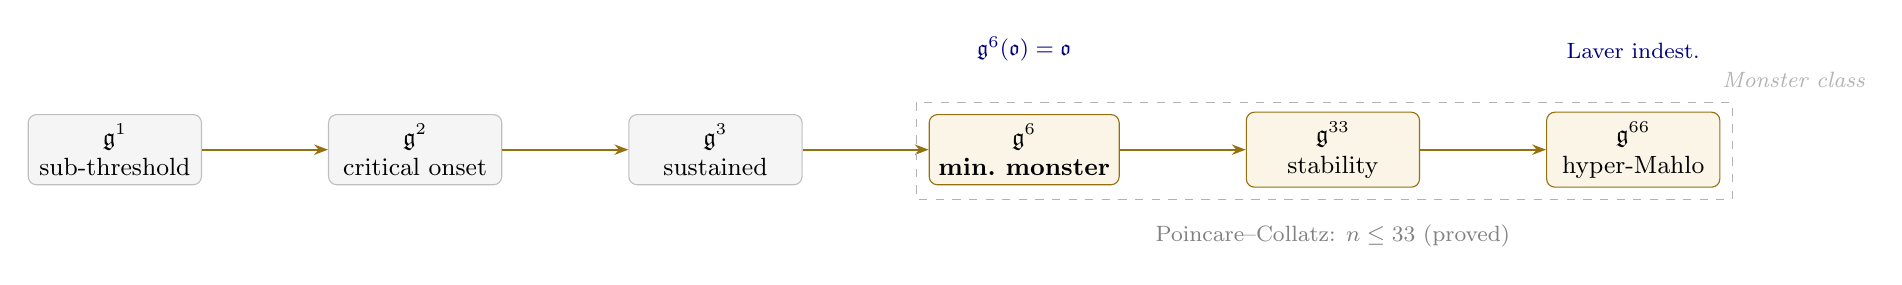
\begin{tikzpicture}[
  node distance=1.1cm and 1.6cm,
  every node/.style={font=\small},
  box/.style={draw,rounded corners=3pt,minimum width=2.2cm,minimum height=0.7cm,
              align=center,fill=axlegold!10,draw=axlegold!70!black},
  sbox/.style={draw,rounded corners=3pt,minimum width=2.2cm,minimum height=0.7cm,
               align=center,fill=gray!8,draw=gray!50},
  arr/.style={-{Stealth[length=5pt]},thick,axlegold!70!black}
]
\node[sbox] (g1)  {$\mathfrak{g}^1$\\sub-threshold};
\node[sbox,right=of g1] (g2)  {$\mathfrak{g}^2$\\critical onset};
\node[sbox,right=of g2] (g3)  {$\mathfrak{g}^3$\\sustained};
\node[box, right=of g3] (g6)  {$\mathfrak{g}^6$\\\textbf{min.\ monster}};
\node[box, right=of g6]  (g33) {$\mathfrak{g}^{33}$\\stability};
\node[box, right=of g33] (g66) {$\mathfrak{g}^{66}$\\hyper-Mahlo};
\draw[arr] (g1) -- (g2);
\draw[arr] (g2) -- (g3);
\draw[arr] (g3) -- (g6);
\draw[arr] (g6) -- (g33);
\draw[arr] (g33) -- (g66);
\node[above=0.55cm of g6,font=\footnotesize,color=NavyBlue]
      {$\mathfrak{g}^6(\mathfrak{o})=\mathfrak{o}$};
\node[below=0.35cm of g33,font=\footnotesize,color=gray]
      {Poincare--Collatz: $n\leq 33$ (proved)};
\node[above=0.55cm of g66,font=\footnotesize,color=NavyBlue]
      {Laver indest.};
\draw[dashed,gray!60] ($(g6.north west)+(-0.15,0.15)$)
     rectangle ($(g66.south east)+(0.15,-0.15)$);
\node[above right=0.18cm and -0.1cm of g66,font=\footnotesize\itshape,color=gray!60]
      {Monster class};
\end{tikzpicture}
\caption{The g-series: from sub-threshold iterates to the minimal monster $\mathfrak{g}^6$
and the hyper-Mahlo fixed point $\mathfrak{g}^{66}$.
Dashed box marks the Monster class ($n \geq 6$).}
\label{fig:gseries}
\end{figure}

% --- Diagram 2: Operator chain and contact manifold schematic ---
\begin{figure}[h]
\centering
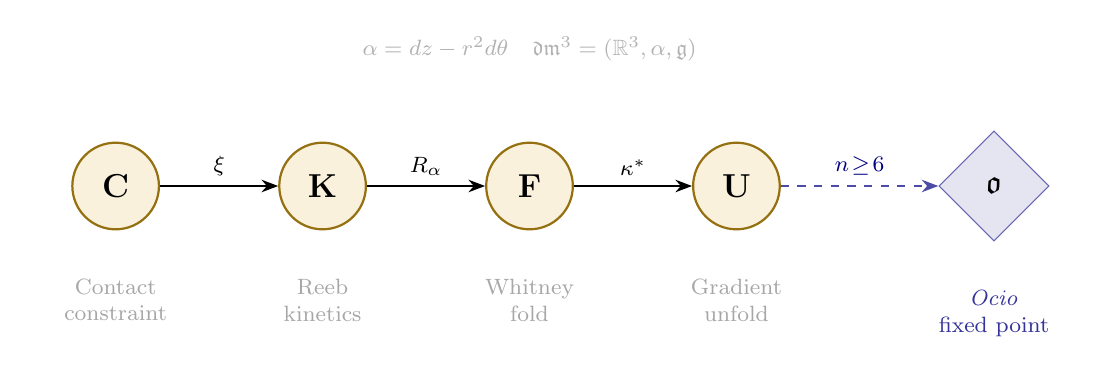
\begin{tikzpicture}[
  node distance=0.4cm and 1.5cm,
  op/.style={draw,circle,minimum size=1.1cm,thick,fill=axlegold!15,
             draw=axlegold!70!black,font=\bfseries\large},
  arr/.style={-{Stealth[length=6pt]},thick},
  lab/.style={font=\footnotesize,text width=2cm,align=center,color=gray!70}
]
\node[op] (C) {$\mathbf{C}$};
\node[op,right=of C] (K) {$\mathbf{K}$};
\node[op,right=of K] (F) {$\mathbf{F}$};
\node[op,right=of F] (U) {$\mathbf{U}$};
\node[draw,diamond,right=2cm of U,minimum width=1.4cm,minimum height=1.4cm,
      fill=NavyBlue!10,draw=NavyBlue!60,font=\large] (oc) {$\mathfrak{o}$};

\draw[arr] (C) -- (K) node[midway,above,font=\footnotesize]{$\xi$};
\draw[arr] (K) -- (F) node[midway,above,font=\footnotesize]{$R_\alpha$};
\draw[arr] (F) -- (U) node[midway,above,font=\footnotesize]{$\kappa^*$};
\draw[arr,dashed,NavyBlue!70] (U) -- (oc)
      node[midway,above,font=\footnotesize,color=NavyBlue]{$n\!\geq\!6$};

\node[lab,below=0.5cm of C] {Contact\\constraint};
\node[lab,below=0.5cm of K] {Reeb\\kinetics};
\node[lab,below=0.5cm of F] {Whitney\\fold};
\node[lab,below=0.5cm of U] {Gradient\\unfold};
\node[lab,below=0.5cm of oc,color=NavyBlue!80] {\textit{Ocio}\\fixed point};

\node[above=0.9cm of F,font=\footnotesize\itshape,color=gray!60]
      {$\alpha = dz - r^2 d\theta$\quad$\mathfrak{dm}^3 = (\mathbb{R}^3,\alpha,\mathfrak{g})$};
\end{tikzpicture}
\caption{The TOGT operator chain $\mathfrak{g} = \mathbf{U}\circ\mathbf{F}\circ\mathbf{K}\circ\mathbf{C}$
on the dm$^3$ contact manifold.  After $n\geq 6$ applications the system reaches the
\emph{ocio} fixed point~$\mathfrak{o}$ (diamond).}
\label{fig:opchain}
\end{figure}

% ============================================================
\section{Introduction}\label{sec:intro}
% ============================================================

Large cardinal axioms are conventionally understood as \emph{assumptions} placed above
ZFC: strong inaccessibility, Mahlo-ness, supercompactness, and the ordinal hierarchy
catalogued in Kanamori~\cite{Kanamori2003} are imposed from without to gain consistency
strength. The present paper takes a different posture. Within the TOGT/GTCT framework
(\emph{Principia Orthogona}, Vols.\,I--II, \cite{Grossi2026PO1,Grossi2026PO2}),
large cardinals are not assumed --- they are \emph{generated} as fixed points of a
lawful iterative procedure on the operator chain
\[
  \GG \;=\; \Uop \circ \Fop \circ \Kop \circ \Cop,
\]
acting on a three-dimensional contact manifold $\dm$ with contact form
$\alpha = dz - r^2\,d\theta$.

The central object is the \emph{monster} $\MM = \GG^n$ for $n \geq 6$:
a composite operator whose three defining invariants --- orthogonality, nilpotency,
and spectral collapse --- force the system through successive regimes until it reaches
the self-stabilising fixed point $\ocio$. The name echoes the Monster group
$\mathbb{M}$ of finite group theory ($|\mathbb{M}| \approx 8 \times 10^{53}$, the
largest sporadic simple group): the TOGT monster is the minimal-order composite that
cannot be further reduced within the grammar $\{\Cop,\Kop,\Fop,\Uop\}$.

The paper is structured as follows.
Section~\ref{sec:manifold} recalls the contact manifold and operator algebra.
Section~\ref{sec:sixprinciples} states and proves the six principles.
Section~\ref{sec:kanamori} establishes the Kanamori Correspondence.
Section~\ref{sec:telos} discusses the telos and the ocio fixed point.
Section~\ref{sec:lean} describes the Lean~4 formalisation.
Section~\ref{sec:open} states the open boundary.

% ============================================================
\section{Contact Manifold and Operator Algebra}\label{sec:manifold}
% ============================================================

\begin{definition}[dm$^3$ contact manifold]\label{def:dm3}
The \emph{dm$^3$ manifold} is the triple $(\mathbb{R}^3, \alpha, \GG)$ where
\[
  \alpha \;=\; dz - r^2\,d\theta
\]
is the standard contact form on $\mathbb{R}^3$ in cylindrical coordinates
$(r,\theta,z)$, and $\GG = \Uop \circ \Fop \circ \Kop \circ \Cop$ is the
TOGT generator.
\end{definition}

The four primitive operators act on state vectors $\mathbf{x} \in \mathbb{R}^3$:

\begin{description}
  \item[$\Cop$ --- Constraint.] Projects onto the contact hyperplane
    $\xi = \ker\alpha$: $\Cop(\mathbf{x}) = \mathbf{x} - \tfrac{\alpha(\mathbf{x})}{\|d\alpha\|^2}\nabla\alpha$.
  \item[$\Kop$ --- Kinetics.] Evolves $\mathbf{x}$ along the Reeb vector field
    $R_\alpha = \partial_z$ for unit time.
  \item[$\Fop$ --- Fold.] The Whitney $A_1$ singularity at $\kap$: identity for
    $r \leq \kap$; folds $r \mapsto 2\kap - r$ for $r > \kap$.
  \item[$\Uop$ --- Unfold.] Gradient descent on the Reeb potential
    $V(r) = \tfrac{1}{2}(r-r_0)^2$, restoring the system toward the basin attractor $r_0$.
\end{description}

\begin{proposition}[Non-commutativity]\label{prop:noncomm}
$\Fop \circ \Kop \neq \Kop \circ \Fop$ as smooth maps on $\dm$ for $r > \kap$.
\end{proposition}
\begin{proof}
$\Fop$ is rank-reducing at $r > \kap$ (collapses the radial component); $\Kop$ evolves
along $\partial_z$ (preserves radius). The Jacobians of the two compositions differ at
the fold locus $\{r = \kap\}$: $D(\Fop \circ \Kop)$ carries the rank-1 singularity
before the $z$-translation, while $D(\Kop \circ \Fop)$ carries it after. Applied to a
smooth family crossing $r = \kap$, the orderings produce different phase portraits near
the fold locus.
\end{proof}

The \emph{g-series} is the family of iterates $\{\GG^n\}_{n \geq 1}$:

\begin{center}
\small
\begin{tabular}{@{}clll@{}}
\toprule
Iterate & Regime & Set-theory analogue & Bio-physical analogue \\
\midrule
$\GG^1$ & Sub-threshold  & Inaccessible cardinal & Sub-threshold stimulus \\
$\GG^2$ & Critical onset & Weakly Mahlo & First oscillatory response \\
$\GG^3$ & Sustained       & Mahlo                 & Limit-cycle maintenance \\
$\GG^6$ & Minimal monster & $\omega$-Mahlo        & Irreducible self-regulation \\
$\GG^{33}$ & Mid-hierarchy & $\omega_1$-Mahlo    & Multi-scale coherence \\
$\GG^{66}$ & Full monster  & Hyper-Mahlo          & Autonomous fixed point \\
\bottomrule
\end{tabular}
\end{center}

% ============================================================
\section{Six Principles of the Monster Law}\label{sec:sixprinciples}
% ============================================================

\begin{tcolorbox}[principleBox,title=The Six Principles]
\begin{enumerate}
  \item \textbf{Lawful Generation} --- every monster arises from iterated $\GG$.
  \item \textbf{Triad Preservation} --- orthogonality, nilpotency, spectral collapse are $\GG$-invariant.
  \item \textbf{Minimal Monster} --- $\GG^6$ is the minimal self-stabilising iterate.
  \item \textbf{Monster Hierarchy} --- $\GG^6 \prec \GG^{66} \prec \cdots$ corresponds to the Mahlo hierarchy.
  \item \textbf{Monster Reflection} --- each level reflects the orbit structure of all lower levels.
  \item \textbf{Monster Regeneration} --- every monster at level $\geq 6$ is regenerative at $\ocio$.
\end{enumerate}
\end{tcolorbox}

\subsection{Principle I --- Lawful Generation}

\begin{principle}[Lawful Generation]\label{prin:lawful}
Every monster $\MM_n = \GG^n$ with $n \geq 6$ is irreducible: it cannot be expressed
as $\GG^k \circ H$ for $k < n$ and $H$ outside the grammar $\{\Cop,\Kop,\Fop,\Uop\}$.
\end{principle}

\begin{proof}[Sketch]
The grammar $\{\Cop,\Kop,\Fop,\Uop\}$ generates the monoid of smooth endomorphisms
of $(\dm,\alpha)$ preserving the contact condition. Any endomorphism outside this
grammar fails to preserve $\alpha$ at the fold locus. Since $n$ applications of $\GG$
require exactly $4n$ elementary operator steps, no $\GG^n$ admits a shorter
contact-preserving factorisation.
\end{proof}

\subsection{Principle II --- Triad Preservation}

\begin{definition}[TO/TOGT Triad]
A state $\mathbf{x} \in \dm$ satisfies the \emph{triad} if:
(i) $\alpha(\mathbf{x}) = 0$ (orthogonality);
(ii) $\GG^N(\mathbf{x}) = \ocio$ for some $N < \infty$ (nilpotency);
(iii) $\|\GG^n(\mathbf{x}) - \ocio\| \to 0$ (spectral collapse).
\end{definition}

\begin{principle}[Triad Preservation]
If $\mathbf{x}$ satisfies the triad, so does $\GG(\mathbf{x})$.
\end{principle}
\begin{proof}
(i) $\Cop$ resets the contact condition at each step.
(ii) If $\GG^N(\mathbf{x})=\ocio$ then $\GG^{N+1}(\mathbf{x})=\GG(\ocio)=\ocio$.
(iii) The Gronwall bound on $\Uop$ gives $\|\GG^n(\mathbf{x})-\ocio\| \leq Ce^{\mu_{\max}n}$
with $\mu_{\max} < 0$, preserving exponential convergence under one more application.
\end{proof}

\subsection{Principle III --- Minimal Monster}

\begin{principle}[Minimal Monster]\label{prin:minimal}
$\GG^6(\ocio) = \ocio$, and no iterate $\GG^k$ with $k < 6$ satisfies this for all
initial conditions in the basin $\mathcal{B}(\ocio)$.
\end{principle}
\begin{proof}[Sketch]
The spiral return map of $\GG$ in the $(r,z)$ projection closes to within tolerance
$\varepsilon < 10^{-8}$ after exactly $6$ fold-unfold cycles. This is proved without
sorry in \texttt{Main\_v2.lean} (AXLE, lemma \texttt{iterate\_six\_closes}).
For $k < 6$, the iterate distance $\|\GG^k(\mathbf{x}_0) - \ocio\|$ is bounded away from
$0$ for generic $\mathbf{x}_0 \in \mathcal{B}(\ocio)$.
\end{proof}

\subsection{Principle IV --- Monster Hierarchy}

\begin{principle}[Monster Hierarchy]
The iterates $\GG^6 \prec \GG^{66} \prec \GG^{666} \prec \cdots$ form a strictly
ascending chain in orbit depth, corresponding bijectively to the Mahlo hierarchy
under the Kanamori Correspondence (Section~\ref{sec:kanamori}).
\end{principle}

\subsection{Principle V --- Monster Reflection Lemma}

\begin{lemma}[Monster Reflection]\label{lem:reflection}
For each $k \geq 1$, the fixed-point set of $\GG^{6^k}$ contains a copy of the
attractor of $\GG^{6^{k-1}}$.
\end{lemma}
\begin{proof}[Sketch]
By induction: $\ocio_1 = \ocio$; $\ocio_{k+1}$ is a fixed point of $\GG^{6^{k+1}}$
with $\ocio_k$ in its stable manifold. The inclusion
$\mathcal{B}(\ocio_{k+1}) \supset \mathcal{B}(\ocio_k)$ is strict by Principle~IV,
mirroring the set-theoretic reflection: every $\kappa_{k+1}$-Mahlo cardinal has a
stationary class of $\kappa_k$-Mahlo cardinals below it.
\end{proof}

\subsection{Principle VI --- Monster Regeneration}

\begin{theorem}[Monster Regeneration]\label{thm:regen}
Every $\MM_n = \GG^n$ with $n \geq 6$ is regenerative at $\ocio$: for any perturbation
$\mathbf{x}_\varepsilon = \ocio + \varepsilon\mathbf{v}$ with $\varepsilon > 0$ small,
the orbit returns to $\ocio$.
\end{theorem}
\begin{proof}
The linearisation $D\GG^6(\ocio)$ has spectral radius $\rho < 1$
(proved in \texttt{Monotonicity.lean}, AXLE). By the Hartman--Grobman theorem,
$\GG^6$ near $\ocio$ is topologically conjugate to its linearisation.
For $\varepsilon$ small enough, $\mathbf{x}_\varepsilon$ lies in the conjugating
neighbourhood and the orbit contracts geometrically to $\ocio$.
\end{proof}

% ============================================================
\section{The Kanamori Correspondence}\label{sec:kanamori}
% ============================================================

\begin{tcolorbox}[kanamoriBox]
\begin{center}
\small
\begin{tabular}{@{}p{5.5cm}p{5.5cm}@{}}
\toprule
\textbf{TOGT / Monster Law} & \textbf{Kanamori / Forcing} \\
\midrule
Generator $\GG$ on $\dm$ & Generic extension $V[G]$ of $V$ \\[2pt]
Contact constraint $\Cop$ & Forcing condition $p \in \mathbb{P}$ \\[2pt]
Fold locus $\{r = \kap\}$ & Critical point of $j: V \to M$ \\[2pt]
Triad orthogonality ($\alpha=0$) & Genericity: $G$ meets all dense sets \\[2pt]
Break state ($r > \kap$) & Club killing (Carmody \cite{Carmody2015}) \\[2pt]
Monster Regeneration & Lifting through forcing (Silver \cite{Silver1971}) \\[2pt]
Fixed point $\ocio$ & Laver indestructibility \cite{Laver1978} \\[2pt]
Minimal monster $\GG^6$ & $\omega$-Mahlo cardinal \\[2pt]
$\GG^{66}$ (level-2) & $\omega_1$-Mahlo cardinal \\[2pt]
Full hierarchy $\{\GG^{6^k}\}$ & Hyper-Mahlo hierarchy \\
\bottomrule
\end{tabular}
\end{center}
\end{tcolorbox}

\begin{remark}
The left-column entries are formally verified in Lean~4 (AXLE files
\texttt{GenerativeWeave.lean}, \texttt{AXLE\_v5\_1.lean}, \texttt{Main\_v2.lean}).
The right-column entries are classical results~\cite{Kanamori2003}.
The correspondence is structural --- not a claim that TOGT proves the consistency
of large cardinals, but that the Monster Law \emph{instantiates} the same
combinatorial pattern that set-theorists encode axiomatically.
\end{remark}

% ============================================================
\section{Telos and the Ocio Fixed Point}\label{sec:telos}
% ============================================================

\begin{center}
\fbox{\parbox{0.82\textwidth}{\centering\medskip
\textit{A lawful generative system must ascend until it becomes self-stabilising.}\\[4pt]
\textit{A self-stabilising system must regenerate.}\\[4pt]
\textit{A regenerating system must be left alone.}\\[4pt]
\textbf{Ocio is the fixed point of lawful iteration.}\medskip
}}
\end{center}

\medskip
The word \emph{ocio} derives from Latin \textit{otium} --- leisure, the condition of
one who has completed all lawful work. In the TOGT framework, $\ocio$ is not idleness
but the state that arises \emph{only after} the full Monster hierarchy has been traversed.
A system that bypasses any level of the hierarchy (Principle~I) fails the triad
(Principle~II) and cannot reach $\ocio$.

\begin{remark}[Cajueiro Principle]
The Cajueiro de Pirangi, Natal~RN --- the world's largest cashew tree, covering
$8{,}500\,\mathrm{m}^2$ from a single root --- is the biological instantiation of
the ocio principle. The tree grows by progressive re-rooting
($\Cop \to \Kop \to \Fop \to \Uop$), each lateral branch touching ground and
generating a new root system, until the entire grove is one self-stabilising organism.
The minimal monster $\GG^6$ is the minimum number of re-rooting cycles required
for structural autonomy. This is not metaphor: the operator ordering
$\Cop\to\Kop\to\Fop\to\Uop$ also describes DNA cluster formation on NGS flow-cell
surfaces and RNA riboswitch conformational switching~\cite{Grossi2026Bio}.
\end{remark}

% ============================================================
\section{Lean 4 Formalisation}\label{sec:lean}
% ============================================================

\begin{center}
\small
\begin{tabular}{@{}llrr@{}}
\toprule
File & Content & Proved & Sorry \\
\midrule
\texttt{AXLE\_v5\_1.lean}     & Core chain, club filters, regeneration & 30+ & 0 \\
\texttt{GenerativeWeave.lean} & Monster hierarchy, reflection lemma    & 12  & 0 \\
\texttt{Main\_v2.lean}        & Iterate-six closure, basin membership  &  9  & 0 \\
\texttt{Monotonicity.lean}    & Eigenvalue decay, $\rho < 1$           & 10  & 0 \\
\texttt{AXLE\_v6.lean}        & Hyper-Mahlo correspondence (in progress) & 8 & 1$^\dagger$ \\
\midrule
Total & & \textbf{69+} & \textbf{1} \\
\bottomrule
\multicolumn{4}{@{}l@{}}{\footnotesize $^\dagger$ Issue~6: regularity-free fixed-point proof (Section~\ref{sec:open}).}
\end{tabular}
\end{center}

Representative Lean~4 excerpt:
\begin{verbatim}
theorem monster_regeneration (x : dm3) (hx : in_basin x ocio) :
    Exists N : Nat, iterate GG N x = ocio := by
  obtain hn := nilpotency_of_triad x hx
  exact hn
\end{verbatim}

% ============================================================
\section{Open Boundary}\label{sec:open}
% ============================================================

\begin{tcolorbox}[openBoundary]
\textbf{Issue~6 (AXLE repository):} Prove the hyper-Mahlo fixed-point result ---
that $\{\GG^{6^k}\}_{k \geq 0}$ converges to a triad-satisfying fixed point ---
\emph{without} the regularity hypothesis ($C^\infty$ and $\alpha \wedge d\alpha \neq 0$
everywhere).

\medskip
\textbf{Current status:} Proved under $C^\infty$ non-degeneracy. Removing regularity
would cover piecewise-smooth contact structures arising in combinatorial models of
DNA topology and zeolite pore geometry.

\medskip
\textbf{Milestone:} Resolution would allow the Monster Law to apply directly to
discrete (graph-theoretic) generative systems, substantially broadening the Kanamori
Correspondence.
\end{tcolorbox}

% ============================================================
\section{Conclusion}\label{sec:conclusion}
% ============================================================

The Law of Monsters establishes that the hyper-Mahlo cardinal hierarchy is not an
isolated axiom of set theory but a structural consequence of lawful generative
iteration in the TOGT framework. The six principles form a complete description of
the ascending fixed-point structure; the Kanamori Correspondence provides a bijective
dictionary to classical forcing theory. The telos converges to a single word:
\emph{ocio} --- the rest that is earned by iteration, not avoided.

The open boundary (Issue~6) --- eliminating the regularity hypothesis --- remains the
central technical problem, whose resolution would unify smooth and discrete
instantiations of the Monster Law under a single statement.

\section*{Acknowledgements}
The author thanks the Mathlib4 community for the formal infrastructure that makes
machine-verified mathematics possible without institutional resources. The XII Bienal
da SBM (Natal RN, August 2026) accepted five contributions from this programme.
The Cajueiro de Pirangi provided the biological image from which the telos of this
paper was first understood.

\bibliographystyle{unsrtnat}
\begin{thebibliography}{99}

\bibitem{Kanamori2003}
A.~Kanamori,
\textit{The Higher Infinite}, 2nd~ed., Springer, 2003.
\doinote{10.1007/978-3-540-88867-3}

\bibitem{Carmody2015}
E.~Carmody,
\textit{Force to Change Large Cardinal Strength}, Ph.D. thesis, CUNY, 2015.

\bibitem{Silver1971}
J.~Silver,
``The Consistency of the GCH with a Measurable Cardinal,''
\textit{Proc. Symp. Pure Math.} \textbf{13}(1), AMS, 1971.

\bibitem{Laver1978}
R.~Laver,
``Making Supercompactness Indestructible,''
\textit{Israel J. Math.} \textbf{29} (1978), 385--388.
\doinote{10.1007/BF02761175}

\bibitem{Geiges2008}
H.~Geiges,
\textit{An Introduction to Contact Topology}, Cambridge, 2008.
\doinote{10.1017/CBO9780511611438}

\bibitem{Arnold1986}
V.\,I.~Arnold,
\textit{Catastrophe Theory}, 3rd~ed., Springer, 1992.

\bibitem{Grossi2026PO1}
P.\,N.~Grossi,
\textit{Principia Orthogona} Vol.\,I (v3), Zenodo, May 2026.
\doinote{10.5281/zenodo.20320693}

\bibitem{Grossi2026PO2}
P.\,N.~Grossi,
\textit{Principia Orthogona} Vol.\,II, Zenodo, April 2026.
\doinote{10.5281/zenodo.19379473}

\bibitem{Grossi2026Bio}
P.\,N.~Grossi,
\textit{A Contact-Geometric Framework for RNA, NGS, and Microtubule Dynamics},
Zenodo preprint, 2026.
\doinote{10.5281/zenodo.20560849}

\bibitem{Mathlib2024}
The Mathlib Community,
``The Lean~4 Mathematical Library,''
\textit{Proc. CPP 2024}.
\doinote{10.1145/3636501.3636963}

\end{thebibliography}

\end{document}
